A significant electronics upgrade to the Ecal was the introduction of large area Hamamatsu S8664-3189 APDs for readout. APDs are ideal for reading out the Ecal modules due to their ability to operate in the fringe magnetic field of the HPS beam line. Both the Institut de Physique Nucleaire d'Orsay (IPN) and Instituto Nazionale di Fisica Nucleare (INFN) groups in the HPS collaboration purchased the large area APDs for upgrade. As the IPN group re-designed the motherboards for the upgrade, INFN developed the testing apparatus so that the gains of each APD could be characterized and sorted into one of 52 high voltage groups to minimize gain variations. The large area APDs are shown in Fig.~\ref{Figure:apd}.

\begin{figure}[H]
  \centering
      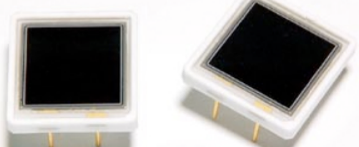
\includegraphics[width=0.4\textwidth]{pics/experiment/apd.png}
  \caption[Hamamatsu S8664-3189 large area APDs]{The Hamamatsu S8664-3189 large area APDs.}
  \label{Figure:apd}
\end{figure}

%%%%%Re-word this section-yuck!!
APDs are reverse-biased diodes with an internal high electric field used to multiply the charge carriers through an avalanche mechanism.  The characteristic gain of APDs is highly dependent on the temperature of the environment due to the interaction of the charge carriers with the phonons. The gain is higher for lower temperatures. 
%%%%%%%%%%%%
The APD gains have a linear dependence on both voltage and temperature. Prior to grouping the APDs for installation in the Ecal, each APD was tested and bench marked to check for quality and optimal operating voltage in order to achieve a pre-selected gain of 150. The testing apparatus was designed and installed by the group from INFN as the same procedure was used in the construction of the Forward Tagger \cite{Celentano}. The bench marking apparatus is shown in Fig.~\ref{Figure:apdtest}.

\begin{figure}[H]
  \centering
      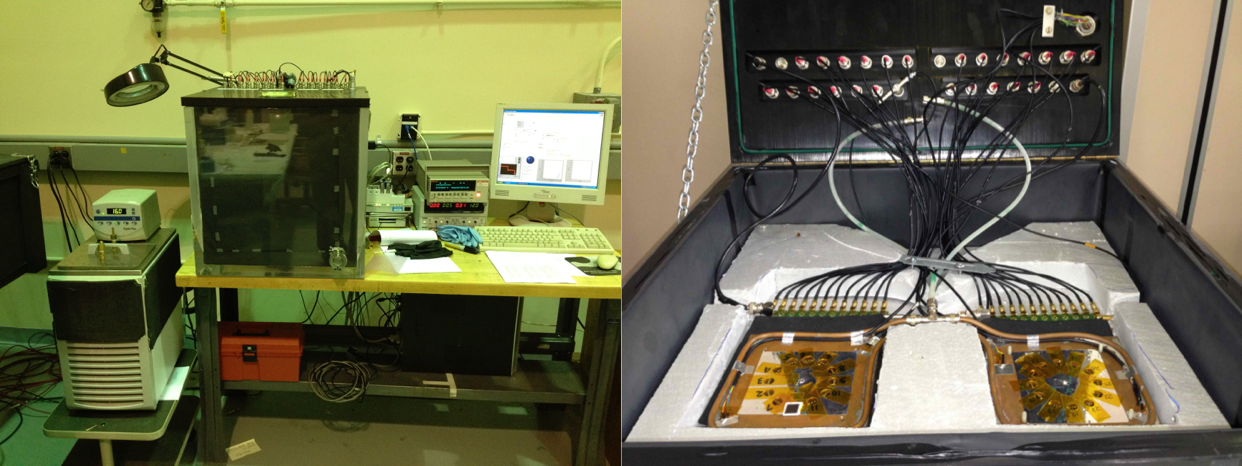
\includegraphics[width=0.7\textwidth]{pics/experiment/apdtests.png}
  \caption[Testing assembly for large area APDs]{On the left, the testing setup is shown and includes a chiller, the light-tight plastic box that contains the LEDs and APDs, an electrometer, and the data acquisition. On the right, the setup inside of the light-tight plastic box is shown that contains a copper cooling plate to maintain the chiller temperature, 10 slots on each side to hold APDs, and the LED in the center of each half.}
  \label{Figure:apdtest}
\end{figure}

In order to avoid condensation on the cooling lines, the temperature range for conducting the tests was limited to 16$\degree$C,18$\degree$C, and 20$\degree$C. During the testing, the current in each APD is measured by the electrometer with the LED on and off while stepping through a range of voltages. The measured dark and light currents for an individual APD during testing are shown in Fig.~\ref{Figure:apdcurrent}.

\begin{figure}[H]
  \centering
      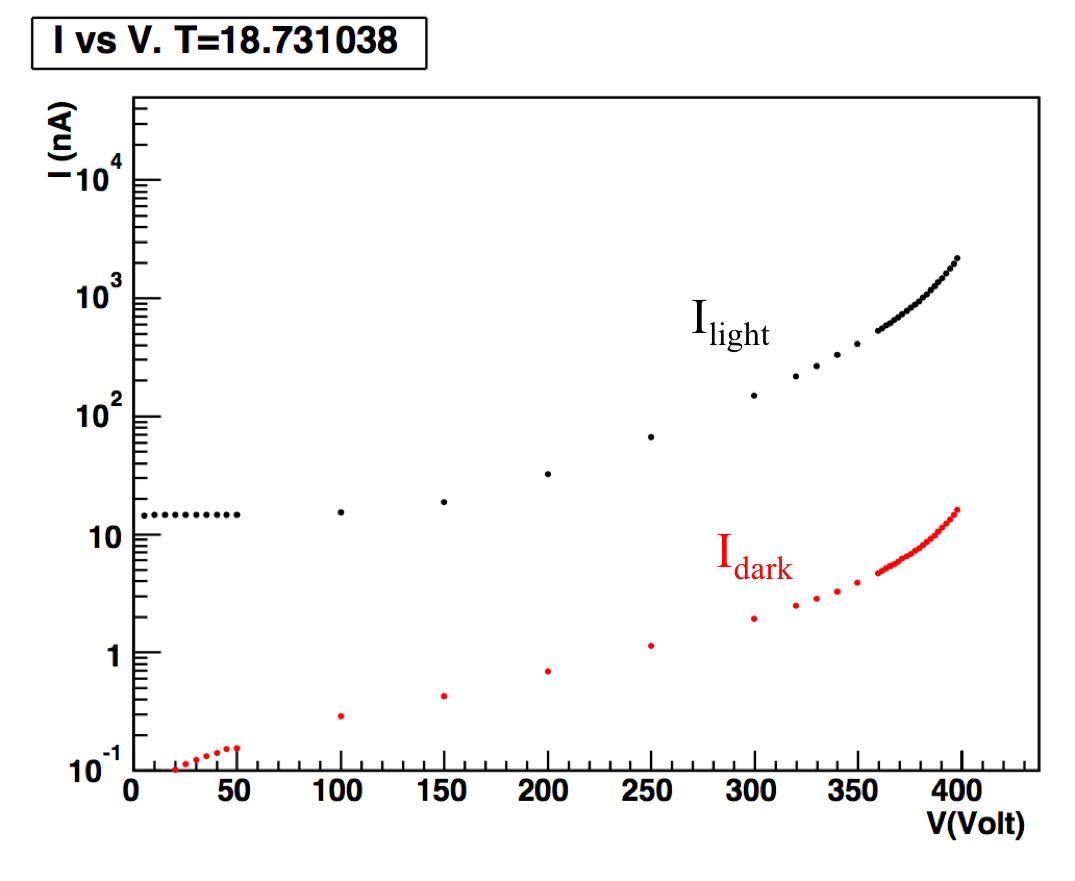
\includegraphics[width=0.4\textwidth]{pics/experiment/apdcurrent.png}
  \caption[APD current draw versus voltage with LED on and off]{The current measured from an individual APD as tested over a range of voltages with both the LED on and off. The measured temperature at the APD for this particular measurement was 18.7~$\deg$C.}
  \label{Figure:apdcurrent}
\end{figure}

The full characterization of the APD gain is calculated by the following relation:

\begin{equation}
	\label{eq:apdgain}
	Gain = \dfrac{I_{light}(V)-I_{dark}(V)}{I_{light}(G=1)-I_{dark}(G=1)} 
\end{equation}

The gain is determined to be 1 when the avalanche mechanism is not present. The $I_{light}(G=1)$ in Eq.~\eqref{eq:gain} the corresponding light current and $I_{dark}(G=1)$ is the measured dark current when the gain is 1. Using this relation, the gain can be characterized for all measured dark currents and should have a linear relation. This relationship is shown in Fig.~\ref{Figure:apdIvG}.

\begin{figure}[H]
  \centering
      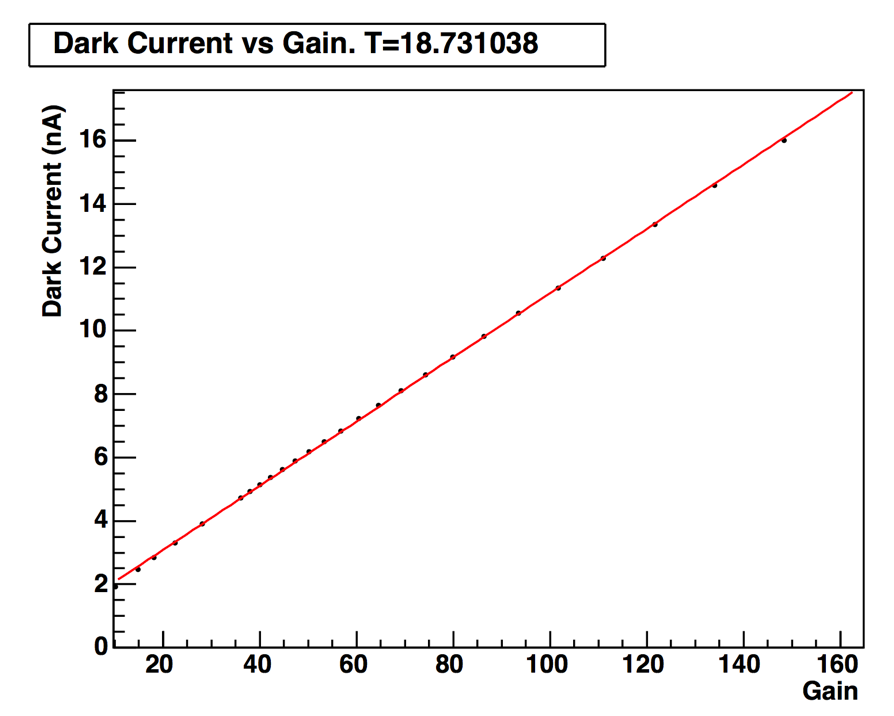
\includegraphics[width=0.4\textwidth]{pics/experiment/apdIvG.png}
  \caption[APD measured dark current as a function of gain]{The current measured from an individual APD as tested over a range of voltages with both the LED on and off. The measured temperature at the APD for this particular measurement was 18.7~$\degree$C.}
  \label{Figure:apdIvG}
\end{figure}

If the relationship between the dark current and the gain is not linear, as shown in Fig.~\ref{Figure:apdIvG}, then the APD was re-tested to ensure quality. In order to appropriately group APDs for common high voltage inputs from the motherboard and minimize gain variations across the Ecal, APDs were placed into 52 common voltage groups ranging from as little as two to maximum ten APDs in each group. The grouping temperature was chosen to be 18~$\degree$C in order to avoid condensation in the cooling lines of the Ecal. The optimal voltage for each APD at 18~$\degree$C and a pre-selected gain of 150 can be extrapolated as shown in Fig.~\ref{Figure:apdTV}.


\begin{figure}[H]
  \centering
      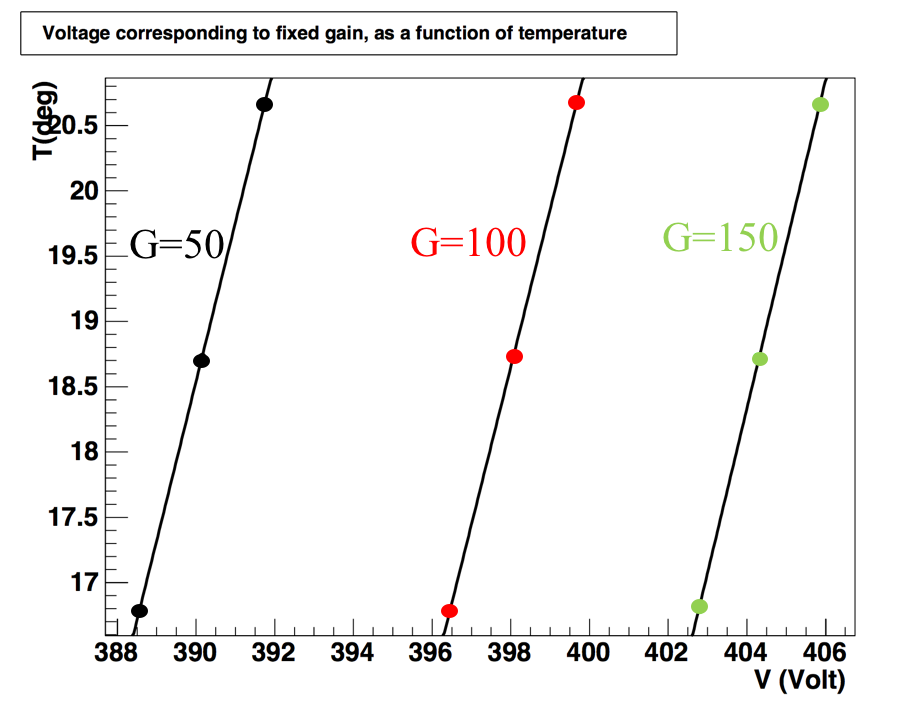
\includegraphics[width=0.4\textwidth]{pics/experiment/apdTV.png}
  \caption[APD fixed gain in terms of voltage and temperature]{The calculated voltages for fixed gains as a function of temperature can be used for group the APDs into appropriate high voltage groups.}
  \label{Figure:apdTV}
\end{figure}
